\begin{figure}[tb]
\centering
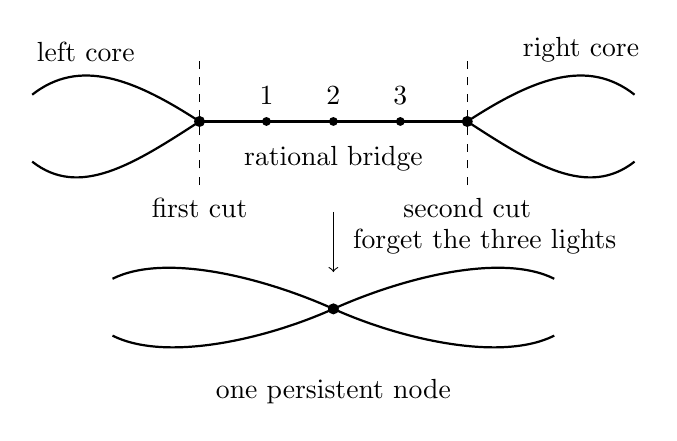
\begin{tikzpicture}[x=.85cm,y=.85cm]
  \draw[thick] (-4.5,.65) .. controls (-3.8,1.2) and (-3,.9) .. (-2,.25);
  \draw[thick] (-4.5,-.35) .. controls (-3.8,-.9) and (-3,-.4) .. (-2,.25);
  \draw[thick] (2,.25) .. controls (3,.9) and (3.8,1.2) .. (4.5,.65);
  \draw[thick] (2,.25) .. controls (3,-.4) and (3.8,-.9) .. (4.5,-.35);
  \draw[thick] (-2,.25) -- (2,.25);
  \fill (-2,.25) circle (2pt);
  \fill (2,.25) circle (2pt);
  \foreach \x/\lab in {-1/1,0/2,1/3}{
    \fill (\x,.25) circle (1.6pt);
    \node[above] at (\x,.36) {$\lab$};
  }
  \draw[dashed] (-2,-.7) -- (-2,1.2);
  \draw[dashed] (2,-.7) -- (2,1.2);
  \node[above] at (-3.7,1.0) {left core};
  \node[above] at (3.7,1.0) {right core};
  \node[below] at (0,.02) {rational bridge};
  \node[below] at (-2,-.75) {first cut};
  \node[below] at (2,-.75) {second cut};
  \draw[->] (0,-1.1) -- (0,-2.0);
  \node[right] at (.15,-1.55) {forget the three lights};
  \draw[thick] (-3.3,-2.1) .. controls (-2.5,-1.7) and (-1,-2.1) .. (0,-2.55);
  \draw[thick] (-3.3,-2.95) .. controls (-2.5,-3.35) and (-1,-3) .. (0,-2.55);
  \draw[thick] (0,-2.55) .. controls (1,-2.1) and (2.5,-1.7) .. (3.3,-2.1);
  \draw[thick] (0,-2.55) .. controls (1,-3) and (2.5,-3.35) .. (3.3,-2.95);
  \fill (0,-2.55) circle (2pt);
  \node[below] at (0,-3.45) {one persistent node};
\end{tikzpicture}
\caption{The two bounding nodes of a light-supported bridge.
After forgetting the lights the bridge contracts.  On a cut chart the
two node conditions contribute two normal cotangent factors.  The same
calculation applies when the two core branches belong to one component.
On the full exceptional surface, coincidence and the bridge class
have integrals $1$ and $2$, respectively, giving
$1-\tfrac12\cdot2=0$.}
\label{fig:bridge-cuts}
\end{figure}
